% Official contribution: https://conferences.iaea.org/event/498/contributions/43617/
% Scheduled date: 2026-10-27.
\paragraph{Abstract}
The objective of this presentation is to provide an overview of the architecture and progress of the new dissemination system, with a focus on the pipelines developed in Python for EXFOR data extraction, alongside with the use of NJOY~\cite{NJOY}, endf-parserpy~\cite{endf-parserpy} and endf-userpy~\cite{endf-userpy} for processing evaluated nuclear data in ENDF-6 format~\cite{ENDF6FormatsManual2023}. These pipelines are designed to extract, process, and store nuclear observables from EXFOR and ENDF into a unified retrieval system, enabling their discovery, visualization and comparison through a common interface.

The system adopts a modular approach that decouples the data processing, storage, retrieval services, and presentation layer, seeking to improve maintainability, scalability, and extensibility.

The presentation will highlight the progress achieved, current challenges, and next steps towards a nuclear reaction data platform that is better aligned with the FAIR principles.


\paragraph{Discussion}
Alejandra Martinez demonstrated the new nuclear data retrieval system, combining experimental and evaluated data into nuclear observables, standardised units and a common interface. The demonstration included filters, library overlays, plot controls and downloads linked to original records. Discussion addressed observable definitions, precomputed and on-demand processing, and provenance in exported data. Participants identified reaction-string interpretation and display utilities as candidates for sharing between centres. Local-agent queries were exploratory; user-upload comparisons and some detailed views are items considered to be developed in the future.

\begin{figure}[H]
    \centering
    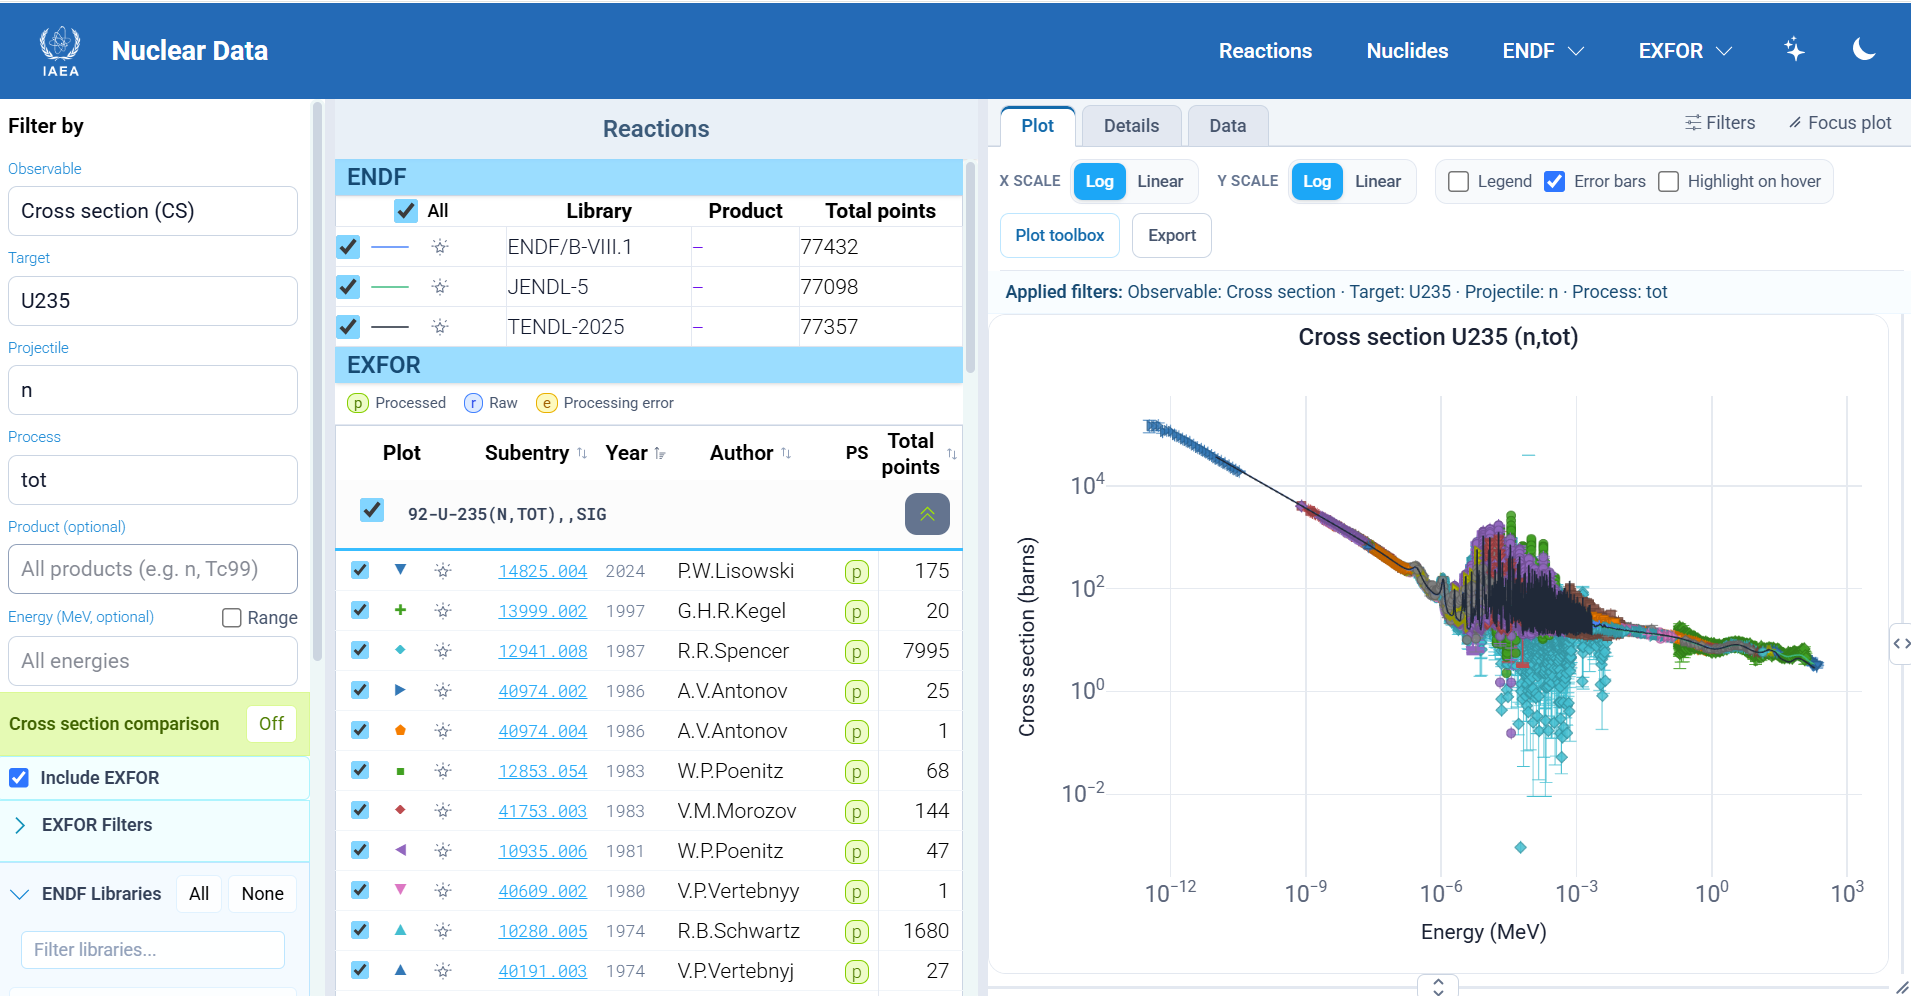
\includegraphics[width=0.75\linewidth]{figures/Screenshot 2026-10-29 144946.png}
    \caption{Screenshot of the New Nuclear Data Web User Interface}
    \label{fig:nuclear-data-web-ui}
\end{figure}

The new development also features modernization of the ENDF Archive user interface with search functions and download capabilities by library, sublibrary and evaluation.

\begin{figure}[H]
    \centering
    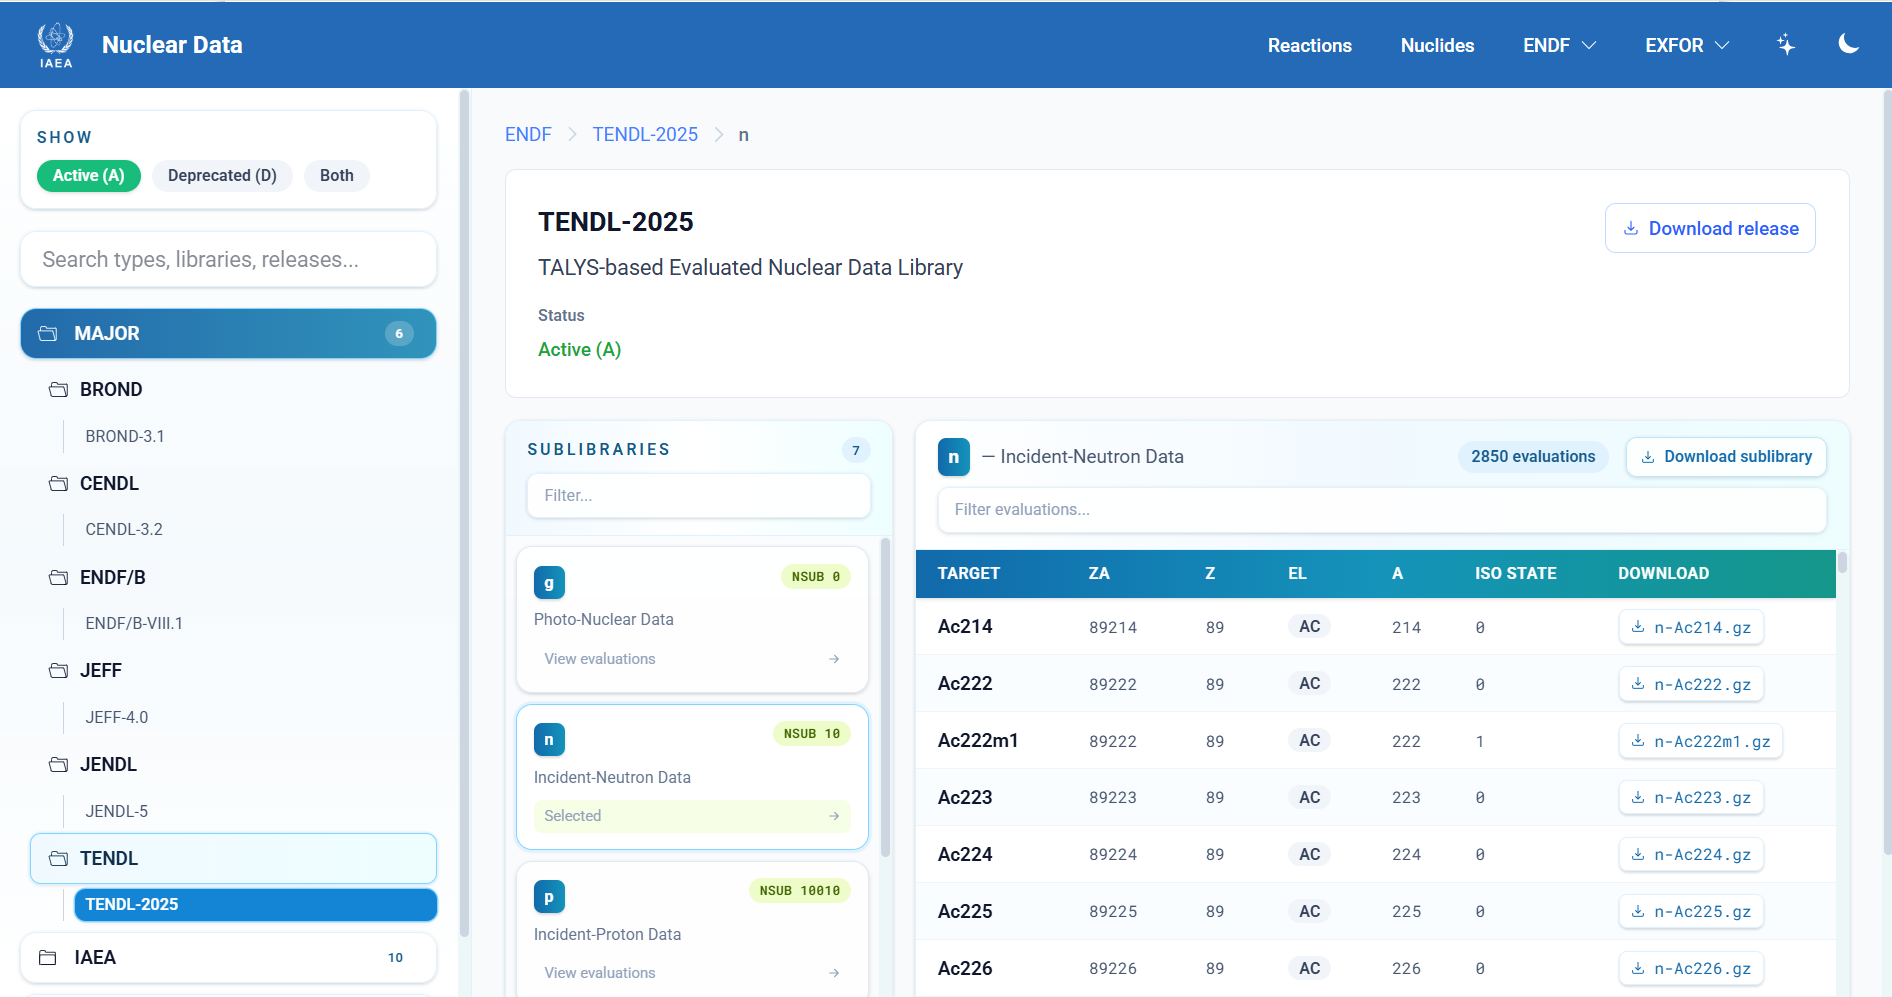
\includegraphics[width=0.75\linewidth]{figures/Screenshot 2026-10-29 145841.png}
    \caption{Screenshot of the New ENDF Archive User Interface}
    \label{fig:endf-archive-ui}
\end{figure}

Another feature that was presented was the inclusion of an AI chat agent aimed to take user questions related to nuclear reactions in natural language and make use of the available APIs and data to answer by giving a result list and plotting the data within the same web user interface or by enabling download of the data and plot images in the chat window.

\begin{figure}[H]
    \centering
    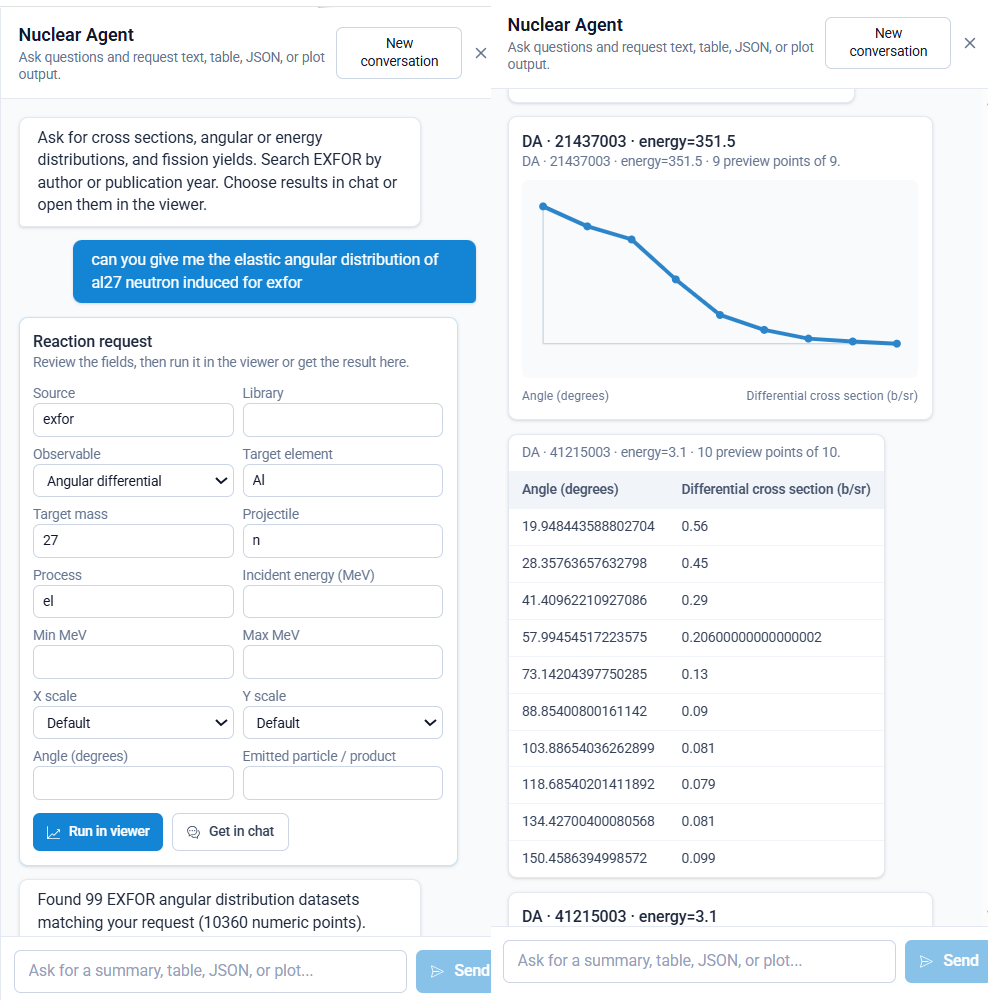
\includegraphics[width=0.75\linewidth]{figures/ai assisstant.png}
    \caption{Screenshot of AI Chat Agent for Experimental and Evaluated Nuclear Data}
    \label{fig:ai-chat-agent}
\end{figure}


